\documentclass{beamer}
\usepackage{amsmath}
\usepackage{amssymb}
\usepackage{graphicx}
\usepackage{caption}
\usepackage{hyperref}
\usepackage[style=numeric,sorting=none,backend=biber]{biblatex}
\addbibresource{bibliography.bib} % Your bibliography file

\usetheme{Madrid} % You can change the theme (e.g., "Berlin", "Copenhagen", "Frankfurt")



% Title, Author, and Date
\title[Impedance Surface Waveguide]{Impedance Surface Waveguide:Theory and Simulation}
\author[]{Mohammad Mahdi Elyasi}
\institute[Amirkabir University of Techonology]{
    Supervisor: Dr. Askarpour \\[1cm] % Professor's Name
    Faculty of Electrical Engineering \\ % Faculty Name
}
\date{\today} % Automatically uses today's date


% Customize the title slide layout
\setbeamertemplate{title page}{
    % Blue strip (Madrid theme)
    \vspace*{-0.5cm} % Adjust vertical spacing
    \begin{beamercolorbox}[wd=\paperwidth,ht=0.4cm,dp=0.2cm,center]{frametitle}
    \end{beamercolorbox}

    % Logo below the strip
    \vspace{0.5cm}
    \centering
    
\includegraphics[width=0.2\textwidth]{amirkabir.png} % Replace with your logo file

    % Title details
    \vspace{0.5cm}
    {\usebeamerfont{title}\inserttitle\par}
    \vspace{0.3cm}
    {\usebeamerfont{author}\insertauthor\par}
    {\usebeamerfont{institute}\insertinstitute\par}
    \vspace{0.3cm}
    {\usebeamerfont{date}\insertdate\par}
}
% Begin Document
\begin{document}


% Title Slide
\begin{frame}
    
    \titlepage
\end{frame}

% Table of Contents Slide
\begin{frame}{Table of Contents}
    \tableofcontents
\end{frame}

% Section: Introduction
\section{Introduction}
\begin{frame}{Introduction}
    \textbf{Impedance Surface Waveguides:}
    \begin{itemize}
        \item Structures designed to confine electromagnetic waves along their surfaces.
        \item Characterized by surface impedance \( Z_s \) that controls wave propagation.
    \end{itemize}
\end{frame}

\subsection{Surface Waves}
\begin{frame}{Surface Waves}
    \textbf{Definition:}
    \begin{itemize}
        \item Surface waves are electromagnetic waves that are confined to the interface between two media\cite{R.Quarfoth}.
        \item They decay exponentially perpendicular to the surface, ensuring energy confinement near the interface.
    \end{itemize}
    \textbf{Key Characteristics:}
    \begin{itemize}
        \item Exist in structures where the surface impedance \( Z_s \) supports bound wave modes.
        \item Propagation is tangential to the surface with wavevectors satisfying \( k^2 = k_x^2 + k_z^2 \).
        \item Common in transverse magnetic (TM) modes.
    \end{itemize}
\end{frame}

\begin{frame}{Surface Waves}
    \textbf{Key Equations\cite{sarabandi}:}
\begin{align}
    \psi_1(x, z) &= A e^{-\nu x} e^{i\beta z}, \\
    \beta^2 - \nu^2 &= k^2, \\
    E_z(x, z) &= -\nu^2 e^{-\nu x} A e^{i\beta z}, \\
    H_y(x, z) &= -i \omega \epsilon \nu A e^{-\nu x} e^{i\beta z}, \\
    \frac{E_z}{H_y} &= Z_s, \\
    \nu &= i \omega \epsilon Z_s.
\end{align}
\textbf{Surface Impedance Analysis:}
\begin{itemize}
    \item If the surface impedance \( Z_s \) is purely imaginary and inductive (\( Z_s = -iX_i \)):
    \begin{itemize}
        \item \( \nu \) becomes a positive real number.
        \item This ensures exponential decay along \( x \)
    \end{itemize}
\end{itemize}
\end{frame}

\subsection{Structure Used}
\begin{frame}{Structure Used}
    \textbf{High Impedance Guide:}
    \begin{itemize}
        \item The waveguide consists of a high-impedance surface surrounded by two low-impedance regions.
        \item These regions are planar with vacuum above the plane, ensuring wave confinement.
    \end{itemize}
    \textbf{Key Properties:}
    \begin{itemize}
        \item The high-impedance surface supports TM surface waves with controlled propagation characteristics.
        \item Surface impedance is engineered to achieve desired wave confinement and dispersion.
    \end{itemize}
\end{frame}

\begin{frame}{Structure}
    \begin{minipage}{0.48\textwidth}
        \centering
            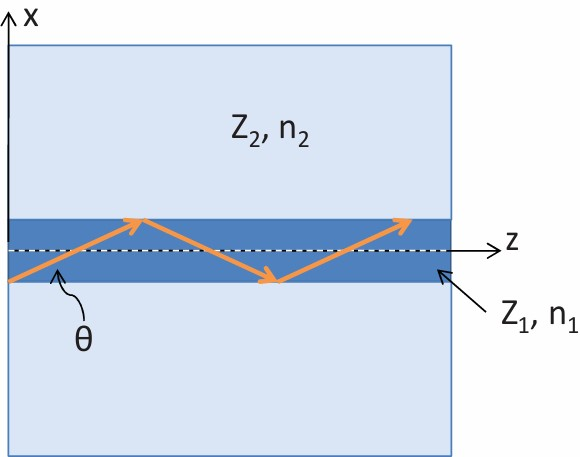
\includegraphics[width=\textwidth]{2.jpg}
            \captionof{figure}{Structre's model}
        \end{minipage}
        \hfill
        \begin{minipage}{0.48\textwidth}
        \centering
            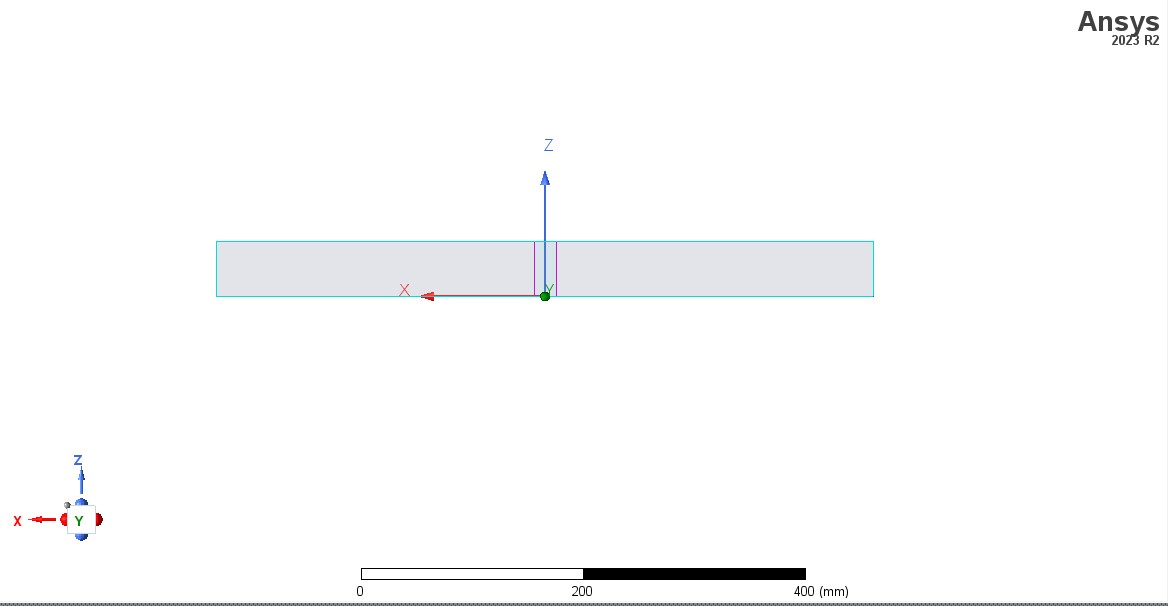
\includegraphics[width=\textwidth]{Top.jpg}
            \captionof{figure}{Structre's model in HFSS}
        \end{minipage}
\end{frame}
% Section: Theory
\section{Theory}
\begin{frame}{Paper's Theory}
    \textbf{Equations:}
    \begin{equation}
        Z_i = Z_0 \sqrt{1 - n_i^2},
    \end{equation}
    proof:
    \begin{align}
        K_x &= K_0 n_i, \\
        K_z &= K_0 \sqrt{1 - n_i^2}.
    \end{align}
    since Propagation is tangential:\\
    \begin{align}
         sin\theta = 1
    \end{align}
    \textbf{Surface Impedance for TM Modes:}
    \begin{align}
        Z_s &= Z_0 \frac{K_z}{K}\\
        Z_s &= Z_0 \sqrt{1 - n_i^2}.
    \end{align}
    
\end{frame}

\begin{frame}{Dispersion Relation and Boundary Conditions}
\textbf{Wavevector Relationship:}
\begin{align}
    K_x^2 + K_y^2 + K_z^2 &= K_0^2.
\end{align}

\textbf{Component Expressions:}
\begin{align}
    K_y &= K_0 \sqrt{1 - n_i^2}, \\
    K_x &= \frac{\pi m + \phi}{d}.
\end{align}

\textbf{Field Continuity Equations:}
\begin{align}
    H_{t,i} + H_{t,r} &= H_{t,t}, \\
    E_{t,i} + E_{t,r} &= E_{t,t}.
\end{align}

\textbf{Surface Impedance Definition:}
\begin{align}
    Z_s &= \frac{E_t}{H_t}.
\end{align}
\end{frame}
\begin{frame}{Wave Propagation in Surface Waveguides}
    
\textbf{Reflection Coefficient and Phase:}
\begin{align}
    R &= \frac{n_1 Z_2 \cos\theta_i - n_2 Z_1 \cos\theta_t}{n_1 Z_2 \cos\theta_i + n_2 Z_1 \cos\theta_t}, \\
    \phi &= \angle(R).
\end{align}

\textbf{Dispersion Equation:}
\begin{align}
    \left( \frac{w n_1}{c} \right)^2 - \left( \frac{\pi m + \phi}{d} \right)^2 - K_z^2 &= 0.
\end{align}
\end{frame}

% Section: Simulation
\section{Simulation and Results}
\begin{frame}{Simulation Overview}
    \textbf{Steps for Simulation:}
    \begin{itemize}
        \item Define the geometry of the waveguide.
        \item Assign the surface impedance \( Z_s \) .
    \end{itemize}
\end{frame}
\begin{frame}{Dispersion}
        \centering
            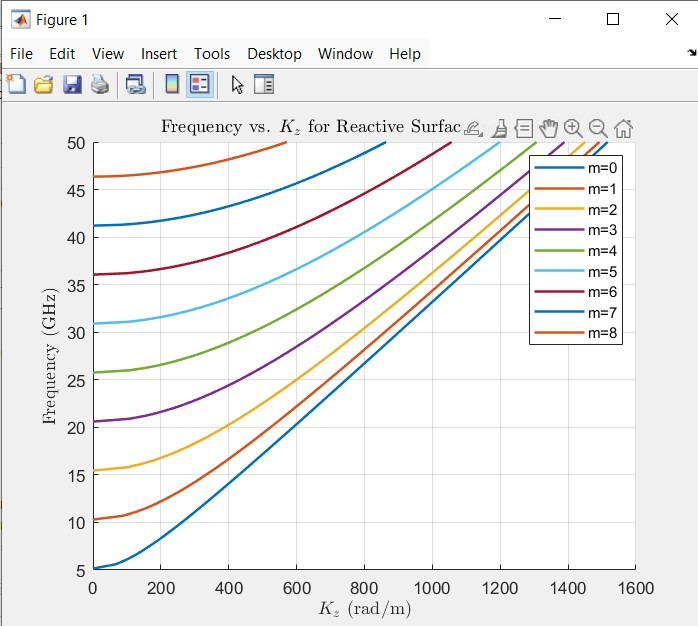
\includegraphics[width=0.6\textwidth]{plot.jpg}
            \captionof{figure}{Dispersion Plot\cite{Github}}
\end{frame}
\begin{frame}{HFSS Results}

        \begin{minipage}{0.48\textwidth}
            \centering
                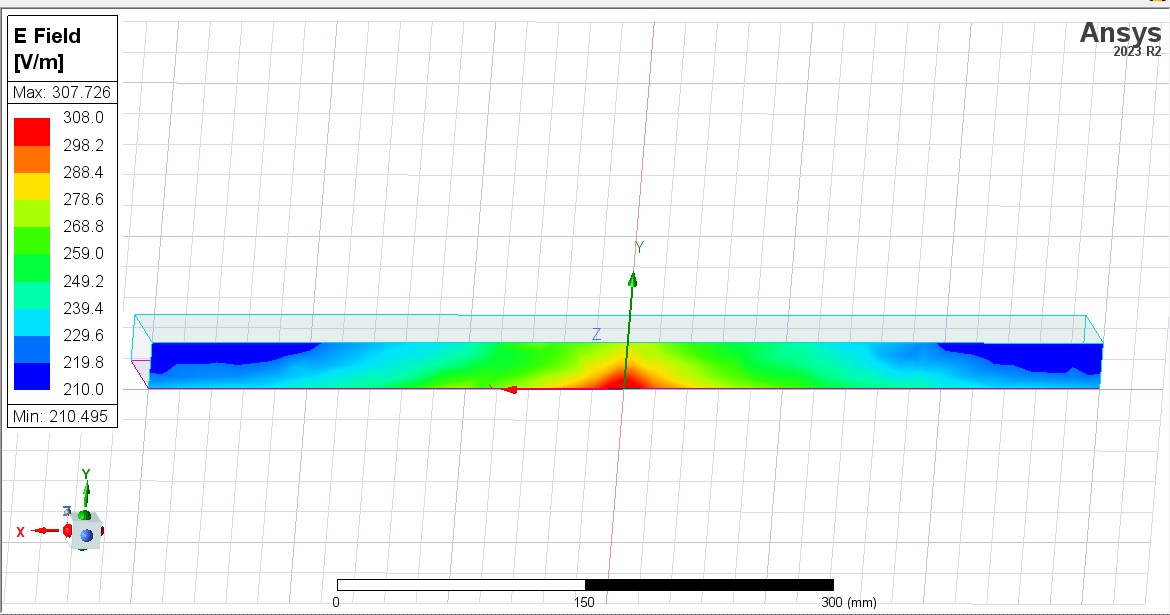
\includegraphics[width=\textwidth]{Mag_E.jpg}
                \captionof{figure}{Magnitude Of Electric Field}
            \end{minipage}
            \hfill
            \begin{minipage}{0.48\textwidth}
            \centering
                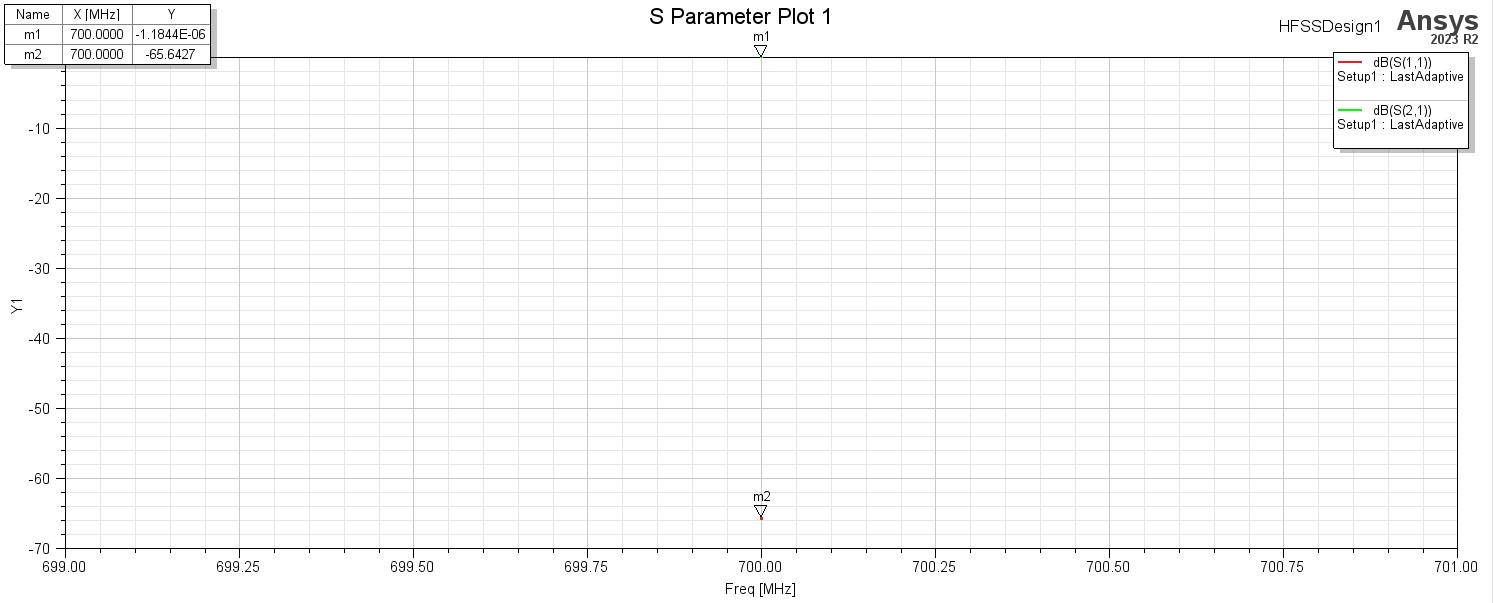
\includegraphics[width=1.2\textwidth]{S11.jpg}
                \captionof{figure}{Scattering Parameters}
            \end{minipage}

\end{frame}
% Section: Conclusion
\section{Conclusion}
\begin{frame}{Conclusion}
    \textbf{Summary:}
    \begin{itemize}
        \item Impedance surface waveguides provide a versatile platform for confining and controlling electromagnetic waves.
        \item Surface impedance \( Z_s \) is critical for waveguide design.
        \item Simulations facilitate detailed analysis and practical implementation.
    \end{itemize}
    
    \textbf{Future Work:}
    \begin{itemize}
        \item Explore advanced materials with tunable \( Z_s \).
        \item Optimize designs for higher frequencies (e.g., THz range).
    \end{itemize}
\end{frame}

% Section 6: References
\section{References}

\begin{frame}
    \printbibliography
\end{frame}


% Section 7: Outro
\begin{frame}{Outro}
    \centering
    {\Large \textbf{Thank you for your attention!}} \vspace{1cm} % Ensures proper centering
    \vfill % Pushes the logo to the bottom
    
\includegraphics[width=0.2\textwidth]{amirkabir.png} % Replace with your logo file
\end{frame}

\end{document}
